% Discovery Philosophy Engineering: Making Philosophical Claims Experimentally Interrogable
% A. H. Bond. Source reconstructed 2026-09-11 from the 2026-09-08 PDF build.
% See PROVENANCE.md for what is verbatim, what was restored, and what is new.
\documentclass[11pt]{article}

\usepackage[letterpaper,margin=1in]{geometry}
\usepackage{lmodern}
\usepackage[T1]{fontenc}
\usepackage[utf8]{inputenc}
\usepackage{amsmath,amssymb,amsthm}
\usepackage{booktabs}
\usepackage{tikz}
\usetikzlibrary{arrows.meta,positioning}
\usepackage[round,authoryear]{natbib}
\usepackage[hidelinks]{hyperref}

\newtheorem{principle}{Principle}
\newtheorem{definition}{Definition}
\newtheorem{proposition}{Proposition}
\newtheorem{conjecture}{Conjecture}
\theoremstyle{remark}
\newtheorem{remark}{Remark}

\title{Discovery Philosophy Engineering:\\ Making Philosophical Claims Experimentally Interrogable}
\author{Andrew H. Bond\\
Department of Computer Engineering, San Jos\'e State University\\
\texttt{andrew.bond@sjsu.edu}}
\date{Draft, September 2026}

\begin{document}
\maketitle

\begin{abstract}
Philosophy is rich in claims about what distinctions matter, what descriptions are
equivalent, what counts as rational or objective, and which structures are fundamental.
Yet many such claims remain insulated from direct empirical pressure because they are
expressed at a level too informal to generate discriminating tests. This paper proposes
Discovery Philosophy Engineering (DPE), a methodology that converts philosophical
conjectures into formal invariance, representation, and boundary claims, compiles those
claims into executable tests, and treats both confirmations and counterexamples as
information about the structure under study. DPE extends Philosophy Engineering from a
one-way discipline, in which philosophical commitments are translated into enforceable
computational constraints, into a closed loop in which the implementation enables
experiments on the commitments themselves. We formalize representation independence by
group actions and quotient maps, define an invariance envelope as the family of
transformations under which a claim survives, and define a boundary witness as a minimal
transformation or intervention that breaks a claimed invariance. A claim is more
fundamental, in the operational sense developed here, when it survives a strictly broader
class of admissible transformations, representations, scales, populations, and domains
without compensating structure added for the purpose. This yields a research protocol.
Formalize, derive invariants, search for low-complexity structure, attack the invariants,
reduce failures to minimal witnesses, and revise the representation or the theory. We
distinguish DPE from experimental philosophy, computational philosophy, automated
scientific discovery, and ordinary formal philosophy, and show how it can use techniques
from each. We illustrate the methodology with five linked artifacts. They are the
Epistemic Invariance Principle, Geometric Evaluation Theory under its own sealed campaign,
a published geometric model of economic behavior whose stake-scaling invariance fails on
independent high-stakes data, Theory Radar, and a discovery line that asked one question
nine times under sealed registrations and ended with one law, one declared scope, and two
recorded boundaries. The failures are not treated as null results. They are localized
boundary measurements that identify missing representational structure. The proposal is
methodological rather than metaphysical. Engineering can make philosophical propositions
experimentally interrogable, and invariance under increasingly severe transformations
gives a disciplined route for finding whatever structure is fundamental.
\end{abstract}

\noindent\textbf{Keywords:} philosophy engineering, experimental philosophy, computational
philosophy, invariance, scientific discovery, representation independence, symbolic
regression, falsification, theory revision, fundamentality

\section{Introduction}

Philosophical inquiry repeatedly asks questions of one form. Which distinctions are real?
Which descriptions are merely different presentations of the same case? Which aspects of a
judgment are objective, and which depend on a standpoint? What is preserved when a problem
is translated, reparameterized, rescaled, or embedded in a richer representation? And when
two theories disagree, which disagreement reflects the world and which reflects the
language in which the world was described?

These are questions about invariance. Physics learned long ago that quantities which
depend on a choice of coordinates can be artifacts of that choice, while structures that
survive admissible transformations are candidates for physical significance. That reading
of geometry as the study of what a group of transformations leaves fixed is
\citet{klein1893}, and its extension to physical law is \citet{weyl1952}.
\citet{nozick2001} made the same move inside philosophy, treating objectivity itself as
invariance under admissible transformations, which is the position this paper turns into a
measurement procedure. Contemporary machine learning likewise treats symmetry and
invariance not merely as useful inductive biases but as objects that can be enforced or
discovered \citep{otto2025}. Causal representation learning has recently been reframed in
a related way, so that identifiability is understood through the preservation of relevant
invariances and symmetries rather than through one fixed causal formalism
\citep{yao2025}.

Philosophy has comparable concerns, but its dominant methods do not compile them into
executable transformation tests. Experimental philosophy has subjected philosophical
judgments and intuitions to empirical study, revealing both stability and fragility in
methods of cases \citep{knobe2024,irikefe2025}. Computational philosophy uses mechanized
methods to extend philosophical analysis and discovery \citep{thagard2024}. Formal
philosophy turns conceptual commitments into mathematical structures. Automated scientific
discovery searches data for compact laws and models, increasingly through symbolic
regression and autonomous closed-loop systems \citep{makke2024,kramer2026}. Each
contributes a necessary piece. None, by itself, supplies a general discipline for taking a
philosophical proposition, compiling it into invariance and boundary claims, attacking
those claims computationally and empirically, and using the resulting witnesses to revise
the philosophy.

This paper proposes such a discipline, Discovery Philosophy Engineering (DPE). It extends
Philosophy Engineering, which defines a method for operationalizing philosophical
commitments through declared equivalences, invariance requirements, canonicalization or
enforcement mechanisms, and machine-checkable audit artifacts \citep{bond2026pe}. The
extension closes the loop. Instead of moving only from a philosophical principle to a
formal constraint to an implementation, DPE uses the implementation to create new
empirical pressure on the principle itself. The route runs from philosophy to
formalization to implementation to probe to witness and back to a revised philosophy. The
governing idea is simple. If a philosophical proposition can be formalized well enough to
implement it, then the implementation often permits experiments on the proposition that
argument alone cannot perform.

The contribution is methodological. It is not a claim that all philosophy should become
experimental or computational. Some philosophical questions are conceptual, normative,
modal, or logical in ways that empirical tests cannot settle. DPE applies where a
philosophical claim entails observable invariance, representation, discrimination, or
boundary structure. Its aim is to identify those entailments sharply enough that both
success and failure become informative.

\section{From Philosophy Engineering to Discovery Philosophy Engineering}

Philosophy Engineering was introduced as the systematic translation of epistemic, ethical,
and logical commitments into computationally enforceable constraints on autonomous systems
\citep{bond2026pe}. Its canonical procedure has four steps. Declare a domain-specific
equivalence relation over representations. Declare what must remain invariant. Implement
canonicalization, quotienting, equivariance, or another enforcement mechanism. Package
transformation trials and witnesses as machine-checkable artifacts. A core example is the
Epistemic Invariance Principle (EIP), which says that a judgment procedure should not
change its conclusion under transformations declared to preserve task-relevant meaning.

DPE generalizes this architecture in the reverse direction. A philosophical claim is
treated as a source of formal commitments that can be interrogated by a transformation
grammar and an empirical observation process. The engineering artifact is not merely the
endpoint of philosophical analysis. It becomes an experimental instrument.

\begin{principle}[Discovery Philosophy Engineering]
A philosophical conjecture is a candidate for Discovery Philosophy Engineering when it can
be translated into at least one non-trivial formal constraint whose satisfaction or
violation is observable under a declared family of transformations, interventions, or
representation changes.
\end{principle}

The requirement of non-triviality is essential. A constant judgment rule is invariant under
every transformation, and it has learned nothing. Philosophy Engineering therefore pairs
invariance with discriminative adequacy. Irrelevant differences must not matter, and
relevant differences must be allowed to matter. DPE inherits that dual obligation.

Figure~\ref{fig:loop} shows the closed loop.

\begin{figure}[t]
\centering
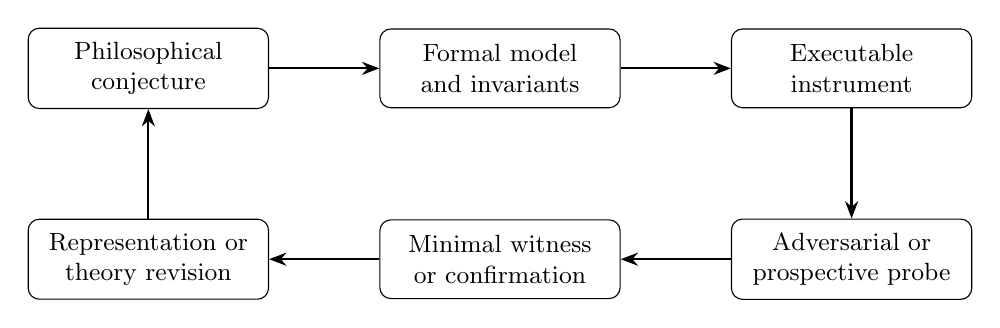
\begin{tikzpicture}[
  node distance=8mm and 14mm,
  box/.style={draw, rounded corners, align=center, inner sep=5pt, font=\small,
              minimum height=10mm, text width=27mm},
  arr/.style={-{Stealth[length=2.2mm]}, thick}]
\node[box] (conj) {Philosophical\\ conjecture};
\node[box, right=of conj] (form) {Formal model\\ and invariants};
\node[box, right=of form] (inst) {Executable\\ instrument};
\node[box, below=14mm of inst] (probe) {Adversarial or\\ prospective probe};
\node[box, left=of probe] (wit) {Minimal witness\\ or confirmation};
\node[box, left=of wit] (rev) {Representation or\\ theory revision};
\draw[arr] (conj) -- (form);
\draw[arr] (form) -- (inst);
\draw[arr] (inst) -- (probe);
\draw[arr] (probe) -- (wit);
\draw[arr] (wit) -- (rev);
\draw[arr] (rev) -- (conj);
\end{tikzpicture}
\caption{Discovery Philosophy Engineering closes the loop between philosophical analysis
and experiment. The output of a failed probe is not only rejection. A reduced
counterexample localizes which distinction or assumption must be revised, which is the
arrow from witness to revision.}
\label{fig:loop}
\end{figure}

\section{Formal Architecture}

\subsection{Representations, transformations, and judgments}

Let $S$ denote a space of world states or cases, $X$ a representation space, and
$\sigma : S \to X$ an encoding map. Let $Y$ be an output space, and let a judgment or
theory-induced prediction be
\begin{equation}
J : X \to \mathcal{P}(Y),
\end{equation}
where $\mathcal{P}(Y)$ is the space of distributions over $Y$ and deterministic judgments
are included as degenerate distributions. Let $\mathcal{T}$ be a set of transformations
$\tau : X \to X$ declared to preserve some target-relevant structure.

The declaration matters. No method can discover relevance without assumptions. An
admissible transformation is not anything we can do to the data. It is a transformation
licensed by the philosophical claim under test. Unit conversion, variable renaming,
permutation of independent premises, paraphrase preserving formal denotation, change of
basis, population transfer, and stake rescaling are different possible transformations
with different semantics.

\begin{definition}[Invariance claim]
Given an output equivalence relation $\sim_Y$, the judgment $J$ is invariant under
$\mathcal{T}$ if
\begin{equation}
J(x) \sim_Y J(\tau x) \qquad \forall x \in X, \ \tau \in \langle \mathcal{T} \rangle,
\end{equation}
where $\langle \mathcal{T} \rangle$ is the closure generated by $\mathcal{T}$ when
composition is meaningful.
\end{definition}

This is the formal core of EIP \citep{bond2026pe}. DPE interprets it as more than a
compliance property. It is an empirically attackable consequence of the underlying
philosophical commitment that the transformations in $\mathcal{T}$ are irrelevant to the
judgment.

\subsection{Quotient structure and representation independence}

Let $x \sim_{\mathcal{T}} x'$ when the two representations lie in the same orbit under the
admissible transformations. The quotient $X / \sim_{\mathcal{T}}$ identifies all
descriptions that the theory says should count as the same case.

\begin{proposition}[Factorization criterion]
If $J$ is constant on every $\sim_{\mathcal{T}}$ equivalence class, then there exists a
well-defined map $\bar{J} : X/\sim_{\mathcal{T}} \to \mathcal{P}(Y)$ such that
$J = \bar{J} \circ q$, where $q : X \to X/\sim_{\mathcal{T}}$ is the quotient map.
\end{proposition}

\begin{proof}
Define $\bar{J}([x]) = J(x)$. Class constancy guarantees that this definition is
independent of the chosen representative. Then $\bar{J}(q(x)) = J(x)$ by construction.
\end{proof}

The proposition is elementary, and its methodological reading is what matters. When a
philosophical theory says that certain differences are merely representational, an
adequate judgment should factor through the quotient that removes them. A failure to factor
identifies a representational dependence.

\subsection{Invariance envelopes}

Binary pass and fail language is too coarse for discovery. A theory may be invariant under
unit changes but not under scale changes, stable across paraphrases but not across
languages, transferable across low-stakes contexts but not across contexts with
consequential stakes. DPE therefore treats invariance as an envelope rather than a
universal predicate.

\begin{definition}[Invariance envelope]
For a theory or judgment procedure $J$ and a universe $U$ of candidate transformations, the
invariance envelope is
\begin{equation}
\mathcal{E}(J) = \{\, \tau \in U \ : \ J(x) \sim_Y J(\tau x) \ \text{over the declared test domain} \,\}.
\end{equation}
\end{definition}

The test domain must be reported, because empirical invariance is always relative to
sampled cases, measurement tolerance, and statistical power. The formal object is an
idealization and empirical work estimates it.

This suggests a partial and operational notion of fundamentality.

\begin{definition}[Comparative fundamentality]
Let $J_1$ and $J_2$ be candidate descriptions with comparable empirical adequacy and
without compensating increases in unconstrained complexity. We say that $J_1$ is more
invariantly fundamental than $J_2$ relative to $U$ if
$\mathcal{E}(J_2) \subseteq \mathcal{E}(J_1)$.
\end{definition}

This is deliberately comparative and local. It does not identify metaphysical
fundamentality with invariance. It says only that, when two descriptions account for the
same target phenomena, the one that survives more meaning-preserving changes has discarded
more representational contingency.

\begin{remark}
The complexity qualification prevents a vacuous victory in which invariance is purchased by
adding a correction for every transformation. DPE therefore pairs invariance breadth with
parsimony, preregistration, and prospective prediction.
\end{remark}

\subsection{Boundary witnesses}

A radar system is useful because a return localizes structure. DPE seeks the analogue for
theories.

\begin{definition}[Boundary witness]
A boundary witness for an invariance claim is a transformation or intervention $\tau^\star$
such that $J(x) \not\sim_Y J(\tau^\star x)$ for some $x$, while no strictly simpler
admissible predecessor under a declared complexity ordering produces the violation.
\end{definition}

For finite transformation grammars, Philosophy Engineering already supplies a witness
principle. Breadth-first search can identify a minimal violating composition under word
length \citep{bond2026pe}. The same reduction is standard practice in software debugging,
where delta debugging narrows a failing input to a minimal failure-inducing core
\citep{zeller2002}, and the methodological content is the same. A failure that has been
reduced says which component is responsible and an unreduced failure does not. DPE
generalizes the idea to continuous parameters by estimating a boundary
\begin{equation}
t^\star = \inf \{\, t \ : \ D\big(J(x), J(T_t x)\big) > \epsilon \,\},
\label{eq:boundary}
\end{equation}
where $D$ is an output discrepancy and $\epsilon$ is a predeclared tolerance. A failed
invariance test then measures where a degree of freedom that was supposed to be irrelevant
begins to matter.

\section{A Protocol for Discovering Fundamental Structure}

DPE organizes research around a repeated sequence of increasingly severe tests, in the
sense of \citet{mayo2018}, where a test counts as severe when the claim would probably have
failed it had the claim been false. The objective is not to maximize the number of
phenomena a theory can be made to fit after the fact. It is to find the smallest structure
that continues to predict after changing everything the theory itself says should not
matter.

\subsection{Stage 1: Formalize the philosophical commitment}

The first step replaces broad language, such as objective, rational, same case, irrelevant
framing, and fundamental, with explicit mathematical commitments. These may take the form
of equivalence relations, group actions, order restrictions, metric identities,
conservation conditions, commutative diagrams, or conditional independences.

Formalization must distinguish at least four statuses. They are definitions, axioms or
modeling assumptions, derived propositions, and empirical hypotheses. This avoids a common
category error in interdisciplinary work, which is treating a convenient representation as
if it were an observed law.

\subsection{Stage 2: Derive high-information consequences}

A good probe is not merely one under which the theory could fail. It is one under which
competing theories diverge sharply. Candidate consequences should therefore be ranked by
expected discriminatory value. Invariance where rivals predict sensitivity, sign reversals,
boundary locations, low-rank constraints, monotonicity, and forbidden orderings are the
useful kinds.

The strongest tests are often consequences the theorist would not have chosen
independently. They are valuable precisely because the formal structure forces them.

\subsection{Stage 3: Search for low-complexity structure}

The discovery engine may be human mathematical reasoning, symbolic regression, equation
discovery, structure learning, or a hybrid. Symbolic regression is attractive because it
searches for concise mathematical relations rather than only for predictive black boxes
\citep{makke2024}. Recent work demonstrates its use for interpretable scientific model
discovery subject to physical constraints \citep{hou2024}, while broader automated science
systems increasingly combine representation learning, equation discovery, experiment
selection, and closed-loop autonomy \citep{kramer2026}.

A DPE search objective can be written schematically as
\begin{equation}
\min_{F \in \mathcal{H}} \ L(F) + \lambda\, C(F) + \mu\, I(F),
\end{equation}
where $L$ is predictive loss, $C$ is structural complexity, and $I$ penalizes instability
under transformations the research program has declared irrelevant. This is not proposed as
a unique objective function. It states the methodological preference for descriptions that
are accurate, simple, and invariant at the same time.

\subsection{Stage 4: Attack the representation}

A candidate law should be deliberately subjected to transformations that preserve
information while changing coordinates or presentation. Basis rotations, unit changes,
equivalent encodings, feature permutations, redundant embeddings, alternative encoders, and
controlled compressions are the usual instruments. If the claimed structure disappears
under an information-preserving change of coordinates, it may be a feature of the
representation rather than of the phenomenon.

This stage is closely aligned with contemporary symmetry discovery. Known symmetries can be
enforced, unknown symmetries can be searched for, and models can be regularized to break
candidate symmetries only when the data require it \citep{otto2025}. DPE imports this logic
as a philosophical test. A distinction should be preserved only if the world forces us to
preserve it.

\subsection{Stage 5: Prospective and cross-domain probes}

After structure discovery, parameters and transformation rules should be frozen as far as
possible. The theory is then evaluated on unseen cases, populations, scales, or domains.
This is the point at which a suggestive reduction becomes evidence of a transferable
structure. Table~\ref{tab:ladder} states the ladder of questions.

\begin{table}[t]
\centering
\small
\begin{tabular}{@{}ll@{}}
\toprule
Level & Question \\
\midrule
Fit & Can the structure describe the observed cases? \\
Perturbation & Does it survive local parameter and data perturbation? \\
Reparameterization & Does it survive information-preserving changes of coordinates? \\
Holdout & Does it predict unseen cases from the same regime? \\
Transfer & Does the same structure survive a different task or population? \\
Cross-domain & Does it organize qualitatively different phenomena? \\
Adversarial probe & Does it survive a deliberately chosen discriminator? \\
Boundary map & Where does it cease to apply, and which assumption breaks? \\
Replication & Can an independent group reproduce the chain? \\
\bottomrule
\end{tabular}
\caption{The ladder of probes, from describing the cases in hand to independent
replication. A result earns only the level it has actually reached, and the level a
program reports is the one a reader should check first.}
\label{tab:ladder}
\end{table}

\subsection{Stage 6: Reduce failures, do not hide them}

A null result may be uninformative. A localized contradiction is not. Once an invariance
fails, DPE seeks the smallest witness and asks which component must absorb the change. The
candidates are the representation, the metric, the constraints, the resolution budget, the
dynamics, and the philosophical equivalence relation itself.

This turns falsification from a binary verdict into structural cartography. The aim is not
to immunize theories against failure. It is to make failure diagnostic.

\section{Relation to Existing Methodologies}

\subsection{Experimental philosophy}

Experimental philosophy applies empirical methods to philosophical questions, particularly
to the distribution and stability of judgments elicited by cases. Its results have forced
methodological scrutiny of intuition-based philosophy, and recent work continues to debate
calibration, comprehension, and robustness to error
\citep{knobe2024,irikefe2025,cova2025}. DPE shares the commitment that philosophical
practice can be empirically interrogated, and its unit of analysis differs. It targets
formal consequences of philosophical theories rather than primarily the psychology of
philosophers or lay participants. Human judgments may be the dependent variable, and so may
physical measurements, algorithmic behavior, economic choices, or theorem-prover outcomes.

\subsection{Computational philosophy}

Computational philosophy uses simulation, automated reasoning, formal modeling, and other
computational techniques to instantiate and extend philosophical research
\citep{thagard2024}. DPE is a narrower methodological proposal within this broad space. Its
distinctive commitment is the closed loop from philosophical conjecture to executable
invariance test to boundary witness and theory revision.

\subsection{Formal philosophy}

Formal philosophy supplies the mathematical language without which DPE would collapse into
metaphor. DPE adds an engineering requirement. Whenever a formal philosophical claim has
observable consequences, the formalism should specify how those consequences are tested and
what would count as a minimal counterexample.

\subsection{Automated scientific discovery}

Automated scientific discovery has advanced from symbolic equation discovery toward
integrated systems capable of selecting experiments, learning representations, and
producing human-interpretable models \citep{kramer2026}. DPE differs in the type of prior
knowledge being compiled. The starting commitments may be philosophical, for example that
renaming should not matter, that equivalent descriptions should receive the same judgment,
or that preference should be derived from evaluator-relative distinctions, and the goal is
partly methodological, which is to determine which of those commitments survive contact
with the world.

\section{Worked Example I: Epistemic Invariance as an Experimental Object}

The Epistemic Invariance Principle states that a judgment should remain equivalent under
meaning-preserving transformations \citep{bond2026pe}. In its original engineering role,
EIP is a specification. A system that changes a medical recommendation because laboratory
results were reordered violates a declared epistemic norm. DPE adds a discovery role.

Suppose a class of transformations $\mathcal{T}$ is proposed as semantically irrelevant.
The engineer can construct a transformation suite, measure judgment discrepancy, and search
for minimal witnesses. Three outcomes are possible.

First, invariance holds across a broad domain. The philosophical claim that the transformed
inputs count as the same case gains operational support. Second, invariance fails because
the model is representation-sensitive even though the philosophical equivalence remains
compelling, and the system is defective relative to the norm. Third, invariance fails
systematically in a way that reveals that the proposed equivalence itself erased a relevant
distinction. In this case the philosophy, and not merely the implementation, should be
revised.

The third outcome is the distinctive DPE case. Engineering exposes a hidden philosophical
assumption by forcing it to encounter concrete counterexamples.

\section{Worked Example II: Geometric Evaluation Theory under its own campaign}

Geometric Evaluation Theory (GET) is an evaluator-relative theory in which states and
actions are mapped into a consequence space, an evaluator supplies a metric and an ideal
point, a finite budget limits the distinctions the evaluator can make, and preference and
choice are derived from those distinctions \citep{bond2026get}. Its foundational draft
separates what the world supplies, the states, the actions, and the consequence map, from
what the evaluator owns, the metric, the budget, and the admissible set. The repository
labels every claim as proved, defined, posited, or open, and grades its predictions through
sealed gates recorded in a campaign file and a claims ledger. Four of its empirical
questions have now been run, across five sealed registrations, and each is an instance of
the loop of Figure~\ref{fig:loop} rather than a promise of one.

The first gate tested the hull law, a consequence of the representation theorem that no
action is strictly worse than every action whose consequences surround it. The consequence
map must be known, so the world was the 1972 American National Election Study, where
respondents placed Nixon, McGovern, Wallace, and the two parties on seven-point issue
scales and rated them on feeling thermometers. The registration was sealed before any
rating was read. On the registered pair of scales 489 respondents had a menu in which the
law could bind, and 50 percent of them violated it at least once, against 66 percent when
each respondent's ratings were shuffled among that respondent's own objects, with no
shuffle in 200 reaching the observed rate. Five other pairs of scales gave the same
ordering. The verdict by the sealed bars was a pass, and the number that matters more than
the verdict is the half. The theorem is deterministic for a representable preference, so
the law holds in this population as a tendency and fails as a law for half of the
respondents. In the language of Section~3 the population is a boundary witness against the
deterministic reading, and what absorbs it is not yet registered, since no error model for
integer placements and integer ratings was part of the seal.

The second gate tested the claim that the indifference threshold of the induced order is
the evaluator's resolution budget. The evaluator was a language model asked how far a value
sits from a target, answering with a number, and three budgets were set independently. They
were the decimals shown, the length in tokens the model was allowed for its report, and the
precision of its weights. A cell's threshold is the gap at which the scorer orders 90
percent of pairs correctly. On fresh pairs every graded threshold sat at 0.87 to 0.88 of
the step the rendering imposed and of the resolution the report length afforded, the
largest ratio 1.15 against a tolerance of 1.5 fixed before the seal, and the constant near
0.87 is where the 90 percent level of a rounding scorer falls, as a self-test on a scorer
with a known grid had shown. The weight precision did not move the threshold at all. Eight
bit and four bit weights left it where full precision put it, to the third digit. Two of
the three declared budgets are resolution budgets and the third is not, which is the
gate's content, and the registration could have carried only the two that worked. What the
gate does not establish is also recorded, which is anything about a human evaluator and
anything about a weight ladder coarse enough to move the threshold, since no such rung was
on the registered ladder. Two instruments tried before the one that ran are kept in the
record rather than discarded. A pairwise chooser read from answer-letter logits was vacuous
when the options straddled the target, because the model simply picks the larger number,
and it had a floor of 7.5 when they did not, from position bias. The reduction of that
failure is a statement about instruments in general. A pairwise chooser measures its own
position bias before it measures a threshold.

The third gate tested the incompatibility theorem, which says that several evaluators
reading one rank-limited representation each pay a regret fixed by their geometries, that a
shared representation best for all of them exists only when their leading subspaces
coincide, and that the least total regret is attained by the leading eigenspace of the
summed geometries. The world was the grouped-query attention of a language model, with the
three query heads of a group as evaluators of one key cache and shared codes of rank 2, 4,
and 8 in 128 dimensions, the read operators recovered from each head alone by the blind
probe of Observation Theory. The first sealed run coded all keys at once and found the
measured attention loss 20 to 330 times the second-order prediction, so the regret formula
was not tested and the verdict was indeterminate. The ordering claim survived on the
measured losses. The leading eigenspace of the summed geometries beat every random code and
the key-covariance code in 32 of 32 cases, while a head's own leading eigenspace was the
best code for that head in fewer than half. The failure was reduced, as Section~4.6
requires. The registered prediction and the registered measurement were not the same
object, a one-key operator against an all-keys loss, and the codes sat far outside the
quadratic regime. A second sealed run measured the object the formula predicts, one key
perturbed by a small isotropic error in the discarded subspace, along a ladder of
perturbation sizes. The ratio of measured to predicted loss was flat in the perturbation
size up to a tenth of a whitened unit and its median over cells was 1.02 to 1.05, so the
recovered operators predict the loss without bias, and 64 draws per cell left a 20 percent
scatter that missed the registered per-triple bar, and that verdict was indeterminate as
well. A seed check with fresh draws showed the scatter to be draw noise. Two errors in that
registration's own error estimate are recorded in it. What the two runs establish together
is the boundary of the theorem's regime. Inside it the regret formula and the bound follow
from the recovered operators, so the only empirical content is whether the loss is
quadratic with the recovered operator, which holds. Outside it the ordering survives and
the private optimum does not. The perturbation ladder is equation~\eqref{eq:boundary}
executed.

The fourth gate tests identification, the theorem that from an evaluator's choices the
metric is recovered up to scale and the ideal up to the metric's kernel, together with its
design bound, that the consequences must span the space affinely. The estimator is the
representation theorem's semidefinite program itself. Two pilots before the seal caught two
wrong drafts of that estimator and showed that the drafted absolute tolerances were empty,
since identification from ordinal data is slow, and the bars were restated on medians
relative to each evaluator's chance level. The sealed run passed in all twelve cells on a
fresh seed. From a weak order on 64 consequences above the dimension the metric and the
ideal's range component were recovered to a few percent of chance, with the error falling
at every step of the battery ladder. At or below the design bound, off the span of a
battery confined to a subspace, and in the kernel of a singular metric, nothing was
recovered. A semiorder that withholds the fifth of pairs closest in distance identified
more slowly. The negative claims, what choices cannot reveal, came out as sharp as the
positive one, and each would have been a witness against the theorem or its remark had it
failed.

GET is suitable for DPE because it makes representation choice explicit. A nine-coordinate
economic representation, a 768-dimensional sentence embedding, or a learned multimodal
latent space could in principle serve as the consequence representation, and the coordinate
labels need not be fundamental. Under an invertible change of basis $z' = Az$ a quadratic
metric transforms as
\begin{equation}
G' = A^{-T} G A^{-1},
\end{equation}
so that
\begin{equation}
z'^{T} G' z' = z^{T} G z .
\end{equation}
The evaluative distance is invariant while the coordinates are not, and the question of
which properties of evaluation survive changes of representation, encoder, dimensionality,
and task is the one the campaign asks gate by gate. The campaign file, the ledger, the
sealed registrations, the run logs, and every result file are in the public repository, and
the encyclopedia entry for the theory carries the numbers with their file and line
citations.

\section{Worked Example III: Economic Stake Invariance as a Radar Return}

A geometric model of economic behavior accepted for publication in IEEE Transactions on
Computational Social Systems provides a useful case because it contains both a successful
reduction and an independent failure \citep{bond2026tcss}. The model represents
alternatives in a nine-dimensional decision space and fits a diagonal Mahalanobis metric.
Structural search selects social impact, virtue and identity, and epistemic status as
active dimensions on the reported benchmark, and the monetary dimension is inactive in the
selected low-stakes calibration.

The important methodological step is not the fit itself but the consequence forced by the
inactive monetary coordinate. Under the share-normalized encoding, positive rescaling of
all monetary stakes should leave predicted offers and rejections unchanged. This produces a
sharp stake-scaling invariance.

The invariance was then tested on individual-level high-stakes ultimatum data from
Meghalaya that played no role in the model's fitting or selection. Offers and rejection
rates changed substantially with stake, and stake retained predictive power even after
conditioning on offer share \citep{bond2026tcss}. The invariance fails.

Under a purely confirmatory view, this is a negative result. Under DPE it is a boundary
measurement. The contradiction identifies a specific missing representational quantity,
because share normalization removes consequential monetary magnitude. An income-relative
monetary coordinate, for example, creates a new testable hypothesis, that decisions depend
on stake relative to local income rather than on nominal stake alone. The sequence runs
from geometry to invariance to independent probe to boundary witness to a new
representation.

This is the sense in which a radar return is not failure. A return is information about
where the current theory stops describing the terrain.

\section{Worked Example IV: Theory Radar as a Discovery Instrument}

Theory Radar is a symbolic-search system that discovers compact classifiers from tabular
data and evaluates whether they can fairly replace ensemble models on the specific dataset
\citep{bond2026radar}. Its architecture combines explicit formula enumeration, search
acceleration, representation augmenters such as PCA or PLS, and held-out replay of the
discovered formula. The repository states that the method's value lies in the comparison
rather than in symbolic formulas always winning. Some datasets admit compact formulas that
match or outperform ensembles, and others do not.

For DPE the relevance is methodological. Theory Radar operationalizes the preference for a
low-complexity explanation without treating simplicity as sacred. A simple formula is
accepted only if it survives fair held-out evaluation. Where the boundary is intrinsically
high-dimensional, the ensemble may win. The negative result is informative because it
identifies a domain in which compression to the searched symbolic grammar loses predictive
structure.

The natural extension is an invariance-aware search objective. Candidate formulas would be
scored not only for predictive performance and syntactic complexity but also for stability
under admissible representation changes. This turns symbolic search into a tool for
discovering not merely simple formulas, but simple formulas whose content survives
transformations that should not matter.

\section{Worked Example V: Nine registrations and one law}
\label{sec:od}

The four examples above each exercise part of the loop. The following line exercises all of
it, nine times, under sealed registrations, and is reported here because it is the only
case in which the protocol of Section~4 ran to its own declared end
\citep{bond2026odline}. It also supplies what the other examples do not, which is a record
of what the protocol costs. Three of the nine registrations failed.

\subsection{The question and the instrument}

A hub is a row of a corpus that appears in many other rows' nearest-neighbour lists. The
instrument counts, for every row, how often it is retrieved among the ten nearest
neighbours of the other rows. The Poisson hub excess is the busiest row's count divided by
the largest count a random assignment of the same retrieval slots would be expected to
reach, so an excess of one is chance. The observer is a linear read of the corpus, a
rotation followed by a diagonal rescaling whose spectrum falls as a power of the index,
with the exponent running from zero, a pure rotation, to two, a reader that sees one
direction. Earlier gates had shown that the hubs of a corpus are made by the reader as much
as by the corpus. The question of this line was whether the amount of hubness is lawful in
the reader's own variables.

The family of laws was declared once and kept. A law is linear in at most three features
drawn from a fixed pool of transforms of variables measured on the observed data. The
search fits every model of the family on the training worlds and ranks by error on held-out
worlds under unseen observer spectra. The pilot freezes the best. The registration is
sealed by renaming the file with the frozen law inside it, the run uses a fresh seed, and a
sealed grader grades. Every bar is a multiple of the frozen law's own pooled pilot error,
fixed before the seal. A competitor beating the law pooled on the transfer groups is a
failure by a clause written in advance.

\subsection{What nine registrations found}

The first four registrations changed the discovery set and kept everything else. The law
changed with the set each time, which is the finding. A law found on Gaussian clouds read
the distance concentration and the spectral dimension and failed off Gaussians. A law found
on seven shape families held every synthetic family and the SIFT descriptors and missed the
Wikipedia embeddings, whose intrinsic dimension of 8 to 20 sat under a spectral dimension
of up to 320. The intrinsic dimension was in the pool and the search had dropped it,
because on full-dimensional families it duplicates the spectral dimension. Putting manifold
worlds into the set made the search take it, and the Wikipedia error fell from 5.3 to 2.5
to 1.0 across the three gates. The discovery set decides the law, and the registry test
written after the third gate says so in one line.

The next two registrations attacked the family rather than the set, and both showed the
same limit. A pool extended with four scale-free tail measures of the neighbour distances
was offered to the search, and the search declined every one of them, an outcome the
registration had named in advance as its first falsification condition. Placing the heavy
tails in the discovery set at the dimensions the transfer asked about then bought the heavy
tails and lost the high-dimensional clouds, and the previously frozen law was the better
predictor pooled, so the gate failed by its own clause. Three registrations had by then put
the same worlds on both sides of one limit. The largest error of every law sat where the
hubness skewness exceeds 12, where a law linear in any transform of the skewness cannot
turn over. The record said the family, and not the set, was the limit.

The seventh registration changed the target and nothing else, predicting the log of the
Poisson hub excess in place of the skewness. On the same 73 worlds and readers the search
froze a law in the concentration of the tenth-neighbour distance, the spectral dimension,
and the intrinsic dimension, with pooled pilot error 0.328, a factor of 1.39 in the excess,
against 1.135 for the nominal formula and 1.598 for chance. On the run it held the heavy
tails, the Gaussian at 512 dimensions, four fresh real slices, and the largest samples at
once, and it beat the nominal formula and chance pooled and inside every group, the first
law of the line to do so. Same family, same pool, same search, same worlds. The target had
been the limit all along.

The eighth registration asked whether the new target takes coverage without paying for it.
It does not. Adding the highest-dimensional clouds to the training set bought every
full-dimensional world beyond 256 dimensions and the best real-slice errors of the line,
and paid on every heavy-tailed world and on an unseen ball, at worse than chance. The
earlier law won pooled and the gate failed. The trade the skewness family had shown
reappeared in the excess family at about a third of the size and with the same sign.

\subsection{The boundary}

Before a ninth registration, an exploration on the rows already collected asked whether any
shape of the declared family holds both sides at once. Twelve configurations were scored
against the frozen law and none passed. The exploration named the mechanism instead. Under
an isotropic reader a uniform ball at 384 dimensions has a tenth-neighbour concentration of
0.003, six times below a Gaussian's at the same dimension, the law's concentration term is
a reciprocal, it diverges there, and it predicts an excess near zero against a truth of
1.4. Removing the reciprocal loses the real corpora, which the reciprocal is what fits.
That is a boundary of the family's shape and not a missing world.

The ninth registration registered that boundary as the claim and searched nothing. A row is
in scope when its tenth-neighbour concentration is at least 0.015, a threshold declared
from the collected rows before the pilot and not moved after it. Inside the scope the
frozen law is claimed within the earlier bars on fresh worlds. Outside it the law is not
claimed, and its pooled error there must exceed the in-scope limit, or else the scope was a
convenience and the claim fails as stated. That second clause is what stops a scope from
being a way of dropping the worlds that fail. The registration also named in advance the
one in-scope cell it expected to lose, a heavy-tailed family at a sample size of 12000,
with the reason, which is that the law carries no term in sample size.

The run held every bar but that one. All eighteen unseen worlds sat inside the limit on
their in-scope rows, pooled 0.31 against a limit of 0.48, the real slices read 0.12 to
0.41, and the law beat both competitors in every group at 0.34 against 1.63 and 1.64. The
180 out-of-scope rows erred at 1.19 against 0.64, which is the second clause holding. The
named cell read 0.67 against 0.64. The verdict was indeterminate, by the named cell and no
other.

\subsection{What the line shows about the protocol}

The standing result is one law with one declared scope and two recorded boundaries. For a
corpus read through a linear observer, on rows whose tenth-neighbour distances vary by at
least 1.5 percent, the log of the busiest row's retrieval count over the Poisson ceiling is
a linear function of the reciprocal of that variation, the log of the spectral dimension,
and the square root of the intrinsic dimension of the observed data, to a factor of about
1.4 in the excess, on every family of world the line built, on corpus slices it never saw,
and at four times its discovery sample. Below 1.5 percent variation the concentration term
diverges and the law is withdrawn. For one heavy-tailed family the law under-predicts by
about a factor of three under the isotropic reader, and a sweep after the line closed
showed this to be a step in sample size between 4000 and 8000 followed by a plateau, which
a law with no term in sample size cannot follow. Neither boundary is repaired by a change
of the discovery set.

Three properties of the protocol are visible in the record rather than asserted. The bars
never moved, and three registrations failed on clauses their own authors had written. Two
pilots froze a law that trailed a competitor on the pilot's own rows, and both were sealed
and run as registered with that fact recorded, because the transfer groups are the test and
the pilot is not. And when a registration that would pass was wanted, the only route the
record allowed was a change of claim, a boundary declared before the run with its risk
named, and the run returned the outcome the risk named. The alternative route, dropping the
worlds that fail without calling that a scope, was available and was not taken.

This is what Definition~4 looks like when it is carried out nine times. Each failure was
reduced to a named cause, each cause was entered as a registry test beside its record, and
the sequence of causes is the finding. The discovery set decides the law. The family cannot
hold both sides of the divide. The target was the limit. Coverage moves the error under the
new target too. The boundary is a divergent term and not a missing world. None of those
five statements was available at the first registration, and each was forced by a failure
that had been reduced rather than absorbed.

\section{The Fundamental Structure Conjecture}

The preceding examples motivate a conjecture rather than a conclusion.

\begin{conjecture}[Fundamental Structure Conjecture]
Many apparently high-dimensional and domain-specific phenomena admit low-complexity
invariant structures acting on richer domain-specific representations, and those structures
can be progressively isolated by searching for what survives admissible changes of
representation, scale, population, and task.
\end{conjecture}

The conjecture is broad and therefore easy to overstate. Three qualifications are
essential.

First, low dimensionality is not guaranteed. Some phenomena may be irreducibly complex at
the scale of interest. Theory Radar's cases in which ensembles decisively outperform
compact formulas are exactly the kind of evidence a serious program must preserve, and so
is the shape boundary of Section~\ref{sec:od}, where the family had no form that held both
sides. Second, invariance is always relative to a transformation class. What survives
translations may fail under changes of scale, and what survives within a culture may fail
across cultures. Third, invariance does not by itself imply ontology. It is evidence that a
structure is less dependent on chosen descriptions, and not a proof that it is
metaphysically ultimate.

The conjecture nonetheless supplies a practical search strategy. Begin with a rich
representation, identify a compact structure, transform the representation, transfer the
structure, and keep only what survives. Repeated quotienting of representational
contingencies can reveal an empirical core that is increasingly difficult to remove without
losing predictive power.

\section{Elegance, Rigor, and the Risk of Beautiful Error}

DPE gives a precise role to two methodological virtues, elegance and rigor. Elegance pushes
toward fewer primitives, reusable structures, and compression across apparently unrelated
phenomena. Rigor prevents elegance from becoming an aesthetic substitute for evidence.

The danger is plain. A mathematically beautiful model can be wrong, and the more beautiful
it is, the easier it may be to rationalize away contrary evidence. DPE therefore treats the
generation of hostile tests as part of the theory rather than as an optional later
exercise. A mature research artifact should include a claim ledger, the distinction between
definitions and measured claims, a registry of admissible transformations, preregistered
gates, holdout data, ablations, and explicit statements of what observations would force
revision. The line of Section~\ref{sec:od} shows what the last of those costs when it is
enforced, which is three failed registrations out of nine.

This discipline is consistent with a pragmatist epistemic stance. The reality of a proposed
structure is not secured by metaphysical assertion. It earns standing by generating
correct, transferable predictions and by surviving increasingly severe attempts to remove
representational artifacts.

\section{Research Program}

A concrete DPE program can be organized into five workstreams.

\subsection{Workstream A: A calculus of philosophical invariants}

Develop a common formal language for philosophical equivalence claims across epistemology,
decision theory, ethics, philosophy of mind, and philosophy of science. Each application
should specify the representation space, the output space, the transformation set, the
output equivalence, non-degeneracy criteria, uncertainty sets, and witness complexity. The
immediate deliverable is a taxonomy of invariance claims, which are exact, approximate,
equivariant, conditional, local, distributional, and scale-dependent.

\subsection{Workstream B: Representation attacks}

Construct benchmark suites in which the same underlying cases are represented through
alternative coordinate systems, embeddings, languages, schemas, and modalities. Candidate
theories should be required to survive invertible transformations and to degrade predictably
under lossy ones. This workstream connects Philosophy Engineering to representation
learning and symmetry discovery.

\subsection{Workstream C: Low-rank evaluation}

Test whether evaluator geometry inferred in one domain transfers to another under
independently determined representations. GET provides a candidate formalism, and the
empirical question should remain open. The decisive experiments fit or identify an
evaluator in one domain, freeze the relevant structure, and predict choices in two others
with minimal target-specific adjustment.

\subsection{Workstream D: Automated theory search}

Extend Theory Radar from classification toward general structure discovery with explicit
complexity and invariance objectives. Candidate outputs include symbolic equations, metric
tensors, low-rank subspaces, transformation groups, and boundary conditions. Search
procedures must replay discovered structures on untouched test data.

\subsection{Workstream E: Boundary atlases}

Instead of publishing only domains where a theory works, construct atlases of where
invariances fail. For each claimed symmetry or equivalence, estimate the boundary in scale,
context, population, or representation at which the effect becomes detectable. These
boundary maps may be more scientifically valuable than a list of successes, because they
name the hidden variables the next theory needs. The two boundaries of
Section~\ref{sec:od}, one in the concentration of a distance and one in sample size, are
entries in such an atlas, and each names a term the next law would have to carry.

\section{Objections and Limitations}

\subsection{This is falsificationism with software}

DPE is compatible with falsificationist virtues and is not exhausted by binary refutation.
Its distinctive object is the structure of the counterexample. Minimal witnesses,
transformation grammars, and boundary estimates turn a failed prediction into information
about which claimed equivalence ceased to hold. The method is closer to debugging a formal
architecture than to recording a single rejected hypothesis \citep{zeller2002}.

\subsection{Invariance does not equal truth}

Correct. A false theory can be invariant, and a true local theory can legitimately fail
under transformations outside its domain. \citet{vanfraassen1989} makes the stronger
version of this objection, that symmetry arguments carry substantive commitments about what
counts as a difference, and DPE accepts it by treating the transformation class as a
declared and contestable object rather than a discovered one. DPE therefore treats
invariance as comparative evidence against representational arbitrariness and not as a
truth criterion. Predictive adequacy, independent replication, and domain specification
remain necessary.

\subsection{The transformation class is chosen by the theorist}

Also correct. This is the central governance problem of any invariance-based method. The
remedy is not to pretend the choice is objective. It is to make the choice explicit,
versioned, contestable, and empirically revisable. Competing philosophical positions can
often be represented as competing transformation registries, and DPE then clarifies where
the disagreement resides. In the programs reported here the registry is a file, it is
sealed before the runs that test it, and Section~\ref{sec:od} gives a case in which the
declared family, and not the data, turned out to be the limit.

\subsection{Philosophical claims are often normative}

Normative claims cannot in general be settled by observing behavior. DPE does not infer an
ought from an is. It can test the operational consequences of a normative principle once
the principle is formalized, which means whether an implementation actually respects
declared equivalences, whether a proposed standard is internally invariant, whether a
policy rule produces representation-dependent outcomes, and whether a normative model
predicts human judgments when it is offered as a descriptive theory.

\subsection{Search will overfit}

Automated search creates severe multiplicity and researcher degrees of freedom. DPE
therefore requires a separation between discovery and evaluation, fair holdout replay,
preregistration where feasible, and independent replication. A symbolic expression found
after searching millions of candidates is not evidence until its search exposure is
accounted for and its performance survives untouched data. The line of
Section~\ref{sec:od} is the worked case. The search ran nine times over one declared
family, every bar was a multiple of a pilot error fixed before the seal, and the two gates
whose frozen law trailed a competitor on the pilot's own rows were run as registered rather
than re-searched.

\section{Discussion: Engineering as an Epistemic Instrument}

The phrase philosophy engineering can sound as if philosophy merely supplies requirements
and engineering implements them. DPE proposes a stronger relationship. Engineering can
expose the hidden commitments of a philosophy by forcing them into interfaces, data
structures, transformation registries, test cases, and failure modes. Ambiguities that
survive prose often become impossible to ignore when a system must decide whether two cases
belong to the same equivalence class.

This changes the epistemic role of implementation. A program is not only a demonstration
that a theory can be instantiated. It can be a measurement instrument for the theory.
Canonicalizers test claims about sameness. Equivariant architectures test claims about
symmetry. Symbolic search tests claims about compressibility. Cross-domain transfer tests
claims about generality. Minimal witnesses test claims about irrelevance. Boundary maps test
claims about scope.

The resulting practice is neither armchair philosophy nor ordinary empirical science. It is
a disciplined traffic between conceptual analysis and experiment. Philosophy proposes
distinctions, mathematics makes the distinctions precise, engineering makes them
executable, experiment pressures them, and philosophy must then explain the returns.

The operational definition of fundamental that follows is modest and useful. Whatever
survives repeated removal of representational contingencies, while preserving discriminative
and predictive adequacy, is a better candidate for fundamental structure than what
disappears under harmless redescription. The search can fail. It may reveal no compact
invariant core. That too is a substantive result.

\section{Conclusion}

Discovery Philosophy Engineering extends Philosophy Engineering from the operationalization
of philosophical commitments to their systematic interrogation. Its central move is to
convert philosophical claims about sameness, relevance, objectivity, rationality,
preference, or fundamentality into explicit transformation and boundary claims. Those claims
can then be implemented, attacked, and revised. The methodology is six verbs. Formalize,
derive, search, probe, witness, revise.

The deepest promise is not that philosophy will be replaced by engineering, nor that every
profound question has a computational answer. It is that some philosophical propositions can
be made precise enough to become experimentally vulnerable. Once that happens,
implementation ceases to be application. It becomes inquiry.

The guiding research question is therefore not whether we have found the fundamental theory.
It is more disciplined. What remains after every distinction that should not matter has been
transformed away, every compact structure has been attacked on unseen data, and every
failure has been reduced to the smallest witness we can find? Whatever survives that process
has earned the right to be taken seriously as fundamental.

\section*{Acknowledgment}

This paper develops and extends concepts introduced in the author's Philosophy Engineering
foundation document, the Geometric Evaluation Theory project, the Theory Radar project, the
Observation Theory campaigns, and the geometric economics research program. The present
manuscript is a methodological synthesis. Empirical claims are attributed to their
originating studies, and every number in Sections 7 and 10 is read from a sealed record in
the repository cited there rather than restated from a draft. The Geometric
Evaluation Theory repository of Section 7 is public. The campaign repository of
Section 10 is not yet, and its records are available on request until it is.

The author used a large language model assistant for source preparation, for drafting
Section~\ref{sec:od} from the sealed campaign records, and for editing. All claims,
verdicts, and numbers were checked against the repository records cited in each section,
and the author is responsible for the content.

\bibliographystyle{plainnat}
\bibliography{refs}

\end{document}
